\documentclass[11pt]{charter}

% El títulos de la memoria, se usa en la carátula y se puede usar el cualquier lugar del documento con el comando \ttitle
\titulo{Sistema de Aislamiento Limitado/Total Ferroviario} 

% Nombre del posgrado, se usa en la carátula y se puede usar el cualquier lugar del documento con el comando \degreename
\posgrado{Carrera de Especialización en Sistemas Embebidos} 
%\posgrado{Carrera de Especialización en Internet de las Cosas} 
%\posgrado{Carrera de Especialización en Intelegencia Artificial}
%\posgrado{Maestría en Sistemas Embebidos} 
%\posgrado{Maestría en Internet de las cosas}

% Tu nombre, se puede usar el cualquier lugar del documento con el comando \authorname
\autor{Ing. Nahuel Espinosa} 

% El nombre del director y co-director, se puede usar el cualquier lugar del documento con el comando \supname y \cosupname y \pertesupname y \pertecosupname
\director{Dr. Ing. Pablo Gomez}
\pertenenciaDirector{CONICET-GICSAFe, FIUBA} 
% FIXME:NO IMPLEMENTADO EL CODIRECTOR ni su pertenencia
\codirector{Mg. Ing. Martín Menendez} % si queda vacio no se deberíá incluir 
\pertenenciaCoDirector{CONICET-GICSAFe, FIUBA}

% Nombre del cliente, quien va a aprobar los resultados del proyecto, se puede usar con el comando \clientename y \empclientename
\cliente{Ing. Alejandro Leonetti}
\empresaCliente{SOFSE}

% Nombre y pertenencia de los jurados, se pueden usar el cualquier lugar del documento con el comando \jurunoname, \jurdosname y \jurtresname y \perteunoname, \pertedosname y \pertetresname.
\juradoUno{Nombre y Apellido (1)}
\pertenenciaJurUno{pertenencia (1)} 
\juradoDos{Nombre y Apellido (2)}
\pertenenciaJurDos{pertenencia (2)}
\juradoTres{Nombre y Apellido (3)}
\pertenenciaJurTres{pertenencia (3)}
 
\fechaINICIO{22 de junio de 2020}		%Fecha de inicio de la cursada de GdP \fechaInicioName
\fechaFINALPlanificacion{22 de agosto de 2020} 	%Fecha de final de cursada de GdP
\fechaFINALTrabajo{21 de junio de 2021}		%Fecha de defensa pública del trabajo final

\begin{document}

\maketitle
\thispagestyle{empty}
\pagebreak


\thispagestyle{empty}
{\setlength{\parskip}{0pt}
\tableofcontents{}
}
\pagebreak


\section{Registros de cambios}
\label{sec:registro}


\begin{table}[ht]
\label{tab:registro}
\centering

\begin{tabularx}{\linewidth}{@{}|c|X|c|@{}}
\hline
\rowcolor[HTML]{C0C0C0} 
Revisión & \multicolumn{1}{c|}{\cellcolor[HTML]{C0C0C0}Detalles de los cambios realizados}     & Fecha      \\ \hline
1.0      & Creación del documento.                                                             & 22/06/2020 \\ \hline
1.1      & Correcciones en las primeras secciones y cambios menores.                           & 14/07/2020 \\ \hline
1.2      & Se agrega gestión del tiempo, recursos humanos y materiales.                        & 27/07/2020 \\ \hline
1.3      & Correcciones en la gestión de recursos, modificaciones en la duración de las tareas & 28/07/2020 \\ \hline
\end{tabularx}
\end{table}

\pagebreak

\section{Acta de constitución del proyecto}
\label{sec:acta}

\begin{flushright}
Buenos Aires, \fechaInicioName
\end{flushright}

\vspace{2cm}

Por medio de la presente se acuerda con el \authorname\hspace{1px} que su Trabajo Final de la \degreename\hspace{1px} 
se titulará ``\ttitle'', consistirá esencialmente en el prototipo de un equipo que permita inhabilitar las señales de 
corte de tracción y frenado de emergencia en el caso de una falla en uno de los subsistemas de seguridad de una 
formación ferroviaria, y tendrá un presupuesto preliminar estimado de 600 hs de trabajo y \$55.000, con 
fecha de inicio \fechaInicioName\hspace{1px} y fecha de presentación pública \fechaFinalName.

Se adjunta a esta acta la planificación inicial.

\vfill

% Esta parte se construye sola con la información que hayan cargado en el preámbulo del documento y no debe modificarla
\begin{table}[ht]
\centering
\begin{tabular}{ccc}
\begin{tabular}[c]{@{}c@{}}Dr. Ing. Ariel Lutenberg \\ Director posgrado FIUBA\end{tabular} &  & \begin{tabular}[c]{@{}c@{}}\clientename \\ \empclientename \end{tabular} \vspace{2.5cm} \\ 
\multicolumn{3}{c}{\begin{tabular}[c]{@{}c@{}} \supname \\ Director del Trabajo Final\end{tabular}} \vspace{2.5cm} \\
\begin{tabular}[c]{@{}c@{}}\jurunoname \\ Jurado del Trabajo Final\end{tabular}     &  & \begin{tabular}[c]{@{}c@{}}\jurdosname\\ Jurado del Trabajo Final\end{tabular}  \vspace{2.5cm}  \\
\multicolumn{3}{c}{\begin{tabular}[c]{@{}c@{}} \jurtresname\\ Jurado del Trabajo Final\end{tabular}} \vspace{.5cm}                                                                     
\end{tabular}
\end{table}

\section{Descripción técnica-conceptual del proyecto a realizar}
\label{sec:descripcion}

Las formaciones ferroviarias cuentan con diferentes sistemas de seguridad a bordo. Los mismos son equipos que se
encargan de supervisar el correcto funcionamiento de los subsistemas críticos. Ejemplos de los mismos son la seguridad
de puertas, el sistema de hombre vivo y la protección de coche a la deriva.

Ante una falla en uno de estos subsistemas, una formación ferroviaria se detiene inmediatamente por la activación 
automática de las señales de corte de tracción y frenado de emergencia. En esta situación el conductor debe llevar a la 
formación a un lugar seguro para que los pasajeros puedan descender y posteriormente a un taller para que pueda ser 
reparada.

En el año 2017, la empresa estatal Trenes Argentinos Operaciones (SOFSE) encargó al CONICET-GICSAFe el desarrollo de un 
equipo que le permita al conductor inhabilitar las señales de corte de tracción (CT) y frenado de emergencia (FE) sin comprometer 
la seguridad de la formación y sus pasajeros. Este equipo se conoce en el ámbito local como Sistema de Aislamiento 
Limitado/Total (SAL/T) y se considera un sistema crítico debido a que, en caso de fallar, puede 
ocasionar daños afectando negativamente la salud de las personas, al medio ambiente y/o generar grandes pérdidas 
materiales.

En el año 2019 se concluyó el desarrollo de un prototipo funcional del SAL/T  en el marco del trabajo de tesis del Ing. 
Ivan Di Vito. En la figura \ref{fig:diagrama_de_bloques} se puede ver cómo interactúa con las señales CT y FE. En modo 
de funcionamiento normal los subsistemas de seguridad tienen conexión directa con el control central. Ante la activación 
por parte del conductor del modo aislado limitado (AL) el SAL/T toma el control de dichas señales.

\begin{figure}[htpb]
\centering 
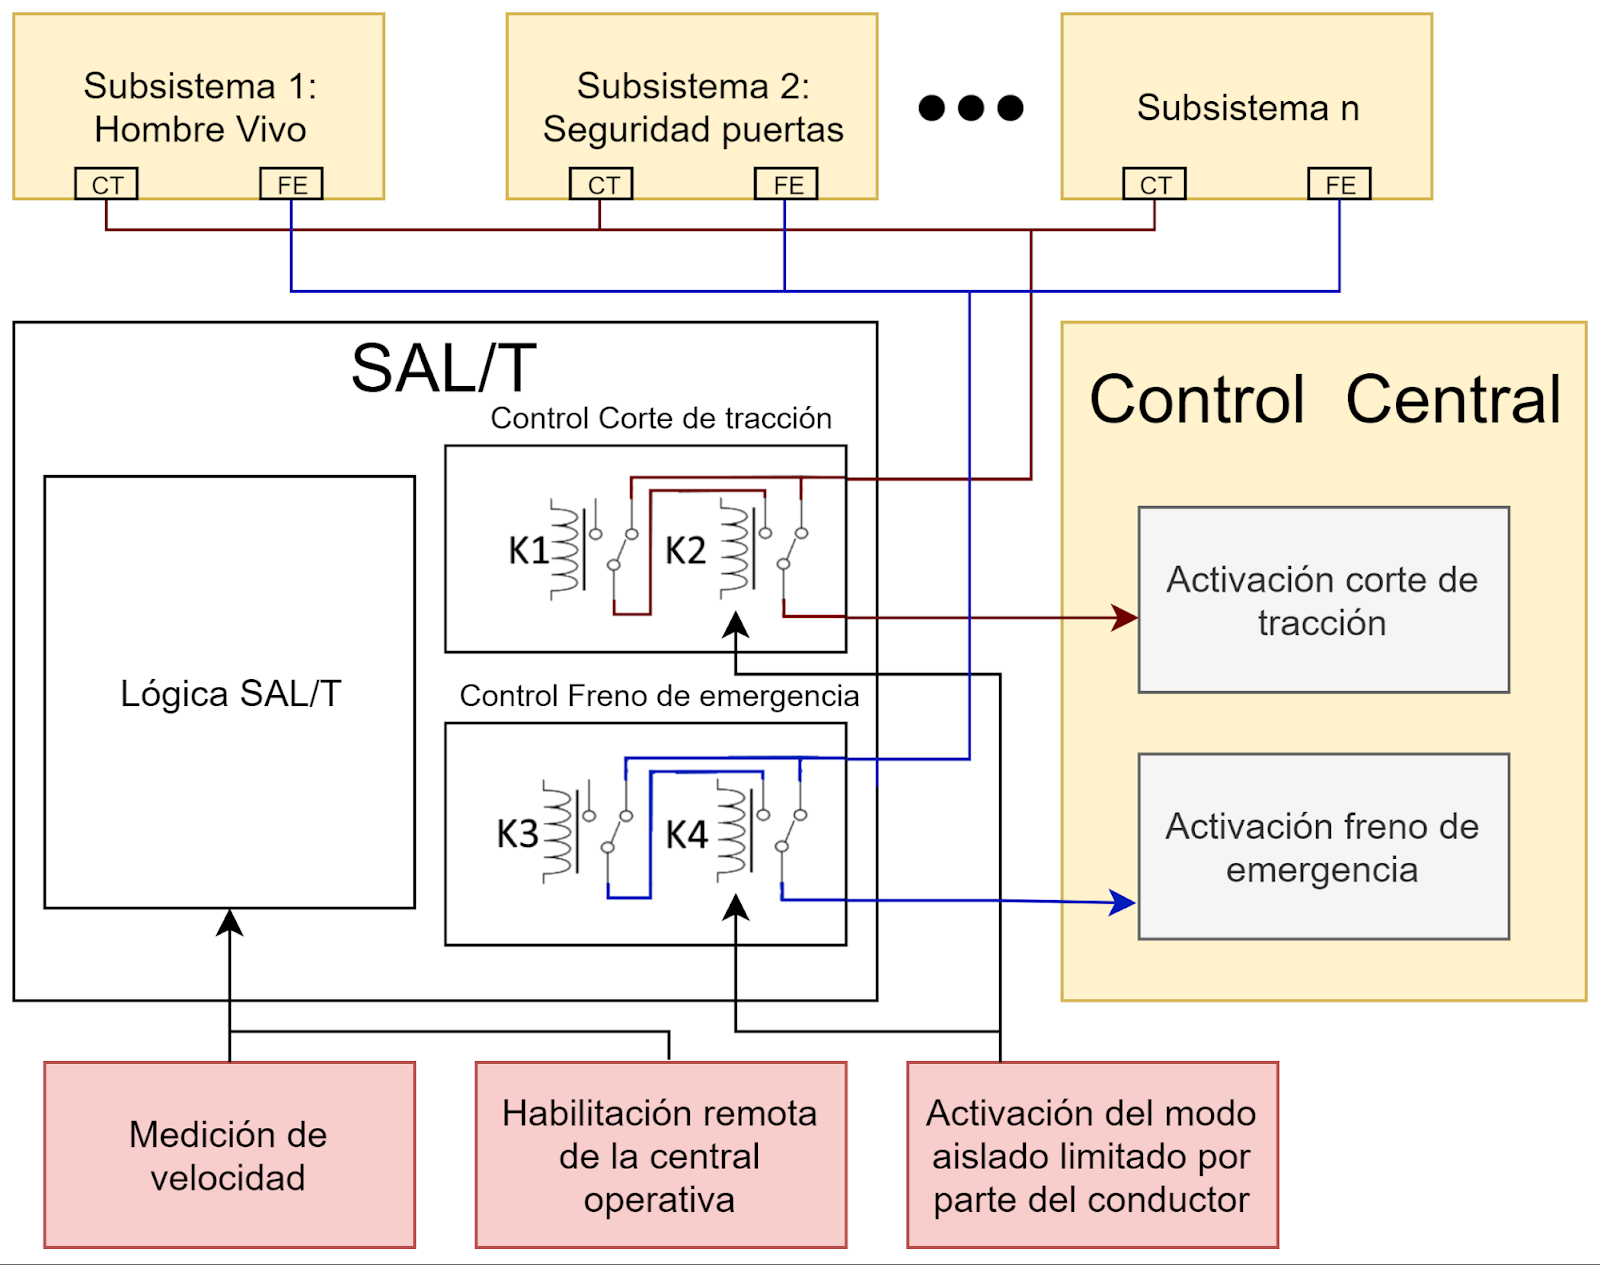
\includegraphics[width=.85\textwidth]{./Figuras/diagrama_de_bloques.png}
\caption{Diagrama conceptual de la interacción del SAL/T con los sistemas de seguridad en una formación.}
\label{fig:diagrama_de_bloques}
\end{figure}

El SAL/T monitorea la velocidad de la formación e informa su estado interno al registrador de eventos Hasler Teloc 1500.
A su vez, se comunica con una central operativa de la cual puede recibir comandos remotos que modifiquen su comportamiento
a través de un enlace redundado.

En la figura \ref{fig:ciclo_de_vida_50126} se resaltan las cinco primeras fases completadas del ciclo de vida propuesto 
por la norma UNE-EN 50126 para aplicaciones ferroviarias. La documentación de la sexta fase, que corresponde al diseño 
e implementación del sistema, y las fases posteriores quedaron fuera del alcance del trabajo original.

\vspace{10px}

\begin{figure}[htpb]
\centering 
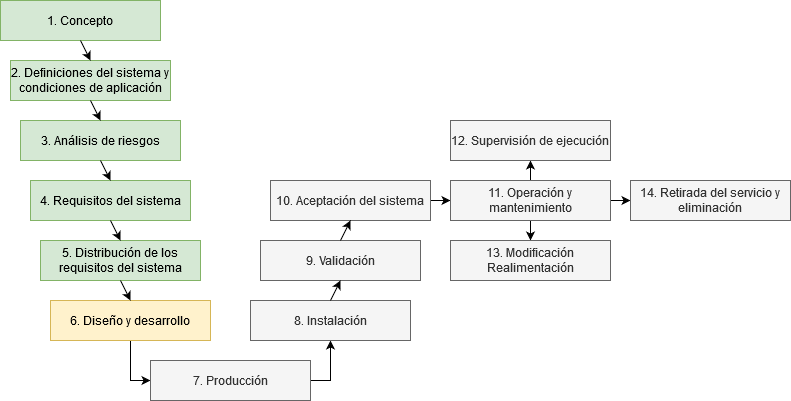
\includegraphics[width=1\textwidth]{./Figuras/ciclo_de_vida_50126.png}
\caption{Ciclo de vida de un sistema propuesto por la norma UNE-EN 50126.}
\label{fig:ciclo_de_vida_50126}
\end{figure}

\vspace{10px}

Este proyecto continuará con el desarrollo del SAL/T revisando los requisitos de seguridad RAMS establecidos en la cuarta fase 
del trabajo original, diseñando subsistemas que se ajusten a los requisitos y verificando el nivel de integridad 
de seguridad (SIL).

Para el caso específico de los sistemas eléctrico-programables (EP) la fase de diseño y desarrollo se divide en dos 
partes relacionadas con el desarrollo del hardware y del software.

\begin{itemize}
\item El diseño del software buscará seguir una metodología acorde a la norma UNE-EN 50128 centrada en la calidad de los 
aspectos de software de los sistemas de ferrocarriles.
\item En el nuevo diseño de la placa principal se reemplazará la plataforma EDU-CIAA-NXP, utilizada como base en la primera 
versión, por un módulo ad-hoc de procesamiento.
\end{itemize}

\newpage

\section{Identificación y análisis de los interesados}
\label{sec:interesados}

\begin{table}[ht]
%\caption{Identificación de los interesados}
%\label{tab:interesados}
\begin{tabularx}{\linewidth}{@{}|l|l|X|X|@{}}
\hline
\rowcolor[HTML]{C0C0C0} 
Rol           & Nombre y Apellido & Organización 	& Puesto 	\\ \hline
Cliente       & \clientename      &\empclientename	& \shortstack[l]{Gerente de Seguridad\\Operacional} \\ \hline
Responsable   & \authorname       & FIUBA        	& Alumno 	\\ \hline
\multirow{2}{*}{Colaboradores} & Dr. Ing. Ariel Lutenberg & CONICET-GICSAFe & \shortstack[l]{Director del Grupo\\de Investigación} \\ \cline{2-4}
& Ing. Sergio Dieleke & SOFSE & \shortstack[l]{Coordinador del\\Laboratorio\\Electrónico\\ - Subgerencia de\\Material Rodante\\Línea Mitre} \\ \hline
\multirow{2}{*}{Orientadores} & \supname & \pertesupname & \shortstack[l]{Director del\\Trabajo Final} \\ \cline{2-4} 
& \cosupname & \pertecosupname &\shortstack[l]{Codirector del\\Trabajo Final} \\ \hline
\end{tabularx}
\end{table}

SOFSE: Operadora Ferroviaria Sociedad del Estado, Trenes Argentinos Operaciones\\
FIUBA: Facultad de Ingeniería, Universidad de Buenos Aires\\
CONICET: Consejo Nacional de Investigaciones Científicas y Técnicas\\
GICSAFe: Grupo de Investigación en Calidad y Seguridad de las Aplicaciones Ferroviarias\\

\newpage

\section{1. Propósito del proyecto}
\label{sec:proposito}

El propósito de este proyecto es continuar el desarrollo de un sistema de supervisión de seguridad de formaciones ferroviarias 
denominado SAL/T (Sistema de Aislamiento Limitado/Total) que alcance niveles RAMS adecuados para su uso a criterio de las autoridades SOFSE y CNRT.

\section{2. Alcance del proyecto}
\label{sec:alcance}

El desarrollo del presente proyecto incluye:

\begin{itemize}
\item Revisión y actualización de la documentación generada en las primeras cinco fases del ciclo de vida del proyecto
original.
\item Diseño, implementación y documentación del firmware siguiendo la norma UNE-EN 50128 utilizando herramientas de integración y ensayos. 
\item Diseño y fabricación de una nueva versión de la placa principal del hardware reemplazando la EDU-CIAA-NXP por un procesador ad-hoc.
\item Estimación del nivel de integridad de seguridad (SIL) del sistema.
\end{itemize}

El presente proyecto NO incluye:

\begin{itemize}
\item Desarrollo de la séptima fase y posteriores del ciclo de vida del proyecto (producción, instalación, validación, etc.).
\item Desarrollo del software necesario para la central operativa.
\item Modificación del gabinete.
\item Certificación de los sistemas a ser desarrollados.
\end{itemize}

\section{3. Supuestos del proyecto}
\label{sec:supuestos}

Para el desarrollo del presente proyecto se supone que:

\begin{itemize}
\item Es posible continuar el proyecto a partir del análisis, la definición de subsistemas e interacciones y el uso de patrones
de diseño del trabajo original.
\item Se tendrá acceso al prototipo actual para hacer pruebas de integridad con el nuevo firmware.
\item Una vez finalizado el diseño del PCB, se podrá fabricar el mismo en un tiempo razonable. 
\item No habrá dificultades para conseguir los componentes electrónicos necesarios.
\item Se adquirirán los conocimientos necesarios sobre la normativa aplicable.
\item El tiempo estipulado será suficiente para alcanzar los objetivos definidos.
\end{itemize}

\section{4. Requerimientos}
\label{sec:requerimientos}

Teniendo en cuenta el estado actual del prototipo y las propuestas para continuar el desarrollo, se detallan los requerimientos
agrupándolos por afinidad. A su vez se indican los códigos de referencia asociados al documento ''R\_DRQ\_10 Distribución de los requisitos del sistema'',
desarrollado durante la quinta fase del ciclo de vida del proyecto, para facilitar su trazabilidad.

\begin{enumerate}
\item Grupo de requerimientos asociados con la interfaz humano-máquina
  \begin{enumerate}
    \item La interfaz debe contar con una llave rotativa precintable para activar el modo aislado limitado. [REQ\_026]
    \item La interfaz debe indicar el estado actual del sistema. [REQ\_012, REQ\_022]
    \item La interfaz debe mostrar la velocidad media del equipo en km/h con 4 dígitos. [REQ\_025]
    \item La interfaz debe indicar el estado de la señal de corte de tracción. [REQ\_019]
    \item La interfaz debe indicar el estado de la señal de freno de emergencia. [REQ\_020]
    \item La interfaz debe indicar la presencia de un comando remoto de la central operativa. [REQ\_021]
    \item La interfaz debe indicar el estado de los módulos GPS. [REQ\_023]
    \item La interfaz debe indicar el estado de la alimentación. [REQ\_018]
  \end{enumerate}
\item Grupo de requerimientos asociados a la comunicación con el registrador de eventos
  \begin{enumerate}
    \item El sistema debe informar al registrador de eventos la activación del modo aislado limitado. [REQ\_008, REQ\_037]
    \item El sistema debe informar al registrador de eventos si la alimentación es correcta. [REQ\_008, REQ\_037]
    \item El sistema debe informar al registrador de eventos la activación del freno de emergencia. [REQ\_008, REQ\_037]
    \item El sistema debe informar al registrador de eventos la activación del corte de tracción. [REQ\_008, REQ\_037]
  \end{enumerate}
\item Grupo de requerimientos asociados a la comunicación con la central operativa
  \begin{enumerate}
    \item El sistema debe informar periódicamente (con un tiempo configurable) su estado a la central operativa a través de la red de datos GPRS, 3G ó 4G. [REQ\_006]
    \item El sistema debe utilizar la antena GPRS/GPS ya disponible en la formación. [REQ\_002]
    \item Debe existir la posibilidad de usar 2 proveedores distintos de datos de manera simultánea. [REQ\_029]
    \item El protocolo de comunicación con la central operativa debe ser MQTT. [REQ\_028]
    \item El sistema debe ser capaz de recibir un comando remoto que anule el corte de tracción y el freno de emergencia bajo cualquier condición (modo aislado total). [REQ\_003]
    \item El sistema debe ser capaz de recibir un comando remoto que active el corte de tracción y el freno de emergencia bajo cualquier condición (modo parada total). [REQ\_003]
    \item El sistema debe ser capaz de recibir un comando remoto que active el corte de tracción y anule el freno de emergencia bajo cualquier condición (modo coche en deriva). [REQ\_003]
    \item El sistema debe ser capaz de recibir un comando remoto que active el corte de tracción y el freno de emergencia de forma intermitente en ciclos de tiempo configurables (modo intermitente). [REQ\_004]
    \item El sistema debe ser capaz de recibir un comando remoto que cancele cualquier comando remoto vigente. [REQ\_003]
    \item El sistema debe ser capaz de recibir comandos remotos que modifiquen sus parámetros internos configurables. [REQ\_004]
    \item Si no se recibe un nuevo comando remoto luego de un tiempo configurable (por defecto 10 segundos, máximo 1 minuto), debe volver al algoritmo de activación de corte de tracción y freno de emergencia por defecto. [REQ\_003]
    \item Ante un comando remoto recibido, debe enviar una confirmación de recepción que permita a la central operativa decidir si es necesaria o no una retransmisión. [REQ\_005]
    \item Debe utilizar algún mecanismo de encriptación para el enlace con la central operativa.
  \end{enumerate}
\item Grupo de requerimientos asociados al modo normal de funcionamiento
  \begin{enumerate}
  \item El modo normal el sistema no debe intervenir en el funcionamiento del material rodante (prioridad alta). [REQ\_010, REQ\_011]
  \item El sistema debe obtener en todo momento la mejor estimación posible de la velocidad de la formación. [REQ\_015]
    \begin{enumerate}
    \item Debe ser capaz de recibir la velocidad a partir de una señal digital provista por el registrador de eventos Hasler Teloc 1500.  [REQ\_007, REQ\_031]
    \item Debe ser capaz de calcular la velocidad a partir de un generador de impulsos ópticos instalado en una o varias ruedas de la formación. [REQ\_009, REQ\_032]
    \item Debe ser capaz de calcular la velocidad a partir de un sistema GPS integrado. [REQ\_027]
    \end{enumerate}
  \item El rango de velocidad soportado por el sistema tiene que estar entre 0 y 120 km/h.
  \item La estimación de velocidad debe tener una precisión del 2\% de fondo de escala. 
  \end{enumerate}
\item Grupo de requerimientos asociados al modo aislado limitado
  \begin{enumerate}
  \item En modo aislado limitado el sistema debe evitar la aplicación del corte de tracción. [REQ\_010]
  \item En modo aislado limitado el sistema debe evitar la aplicación del freno de emergencia. [REQ\_011]
  \item Ante cualquier error interno, el sistema debe dejar de intervenir en la aplicación del corte de tracción. [REQ\_010, REQ\_036]
  \item Ante cualquier error interno, el sistema debe dejar de intervenir en la aplicación del freno de emergencia. [REQ\_011, REQ\_034]
  \item En modo aislado limitado el sistema debe emitir una señal sonora intermitente a través de un buzzer. [REQ\_017]
  \item En modo aislado limitado el sistema debe evitar que la velocidad del material rodante supere una serie de límites configurados. [REQ\_016]
    \begin{enumerate}
    \item Si al pasar de modo normal a modo aislado limitado no se cuenta con una estimación de velocidad, debe activar el corte de tracción y el freno de emergencia por 30 segundos. [REQ\_016]
    \item Si se supera una velocidad configurable (por defecto 30 km/h), debe activar el corte de tracción y emitir una señal sonora continua a través de un buzzer. [REQ\_016]
    \item Si se supera una velocidad configurable (por defecto 36 km/h), debe activar el freno de emergencia. [REQ\_016]
    \item Una vez aplicado, el corte de tracción debe dejar de aplicarse si la velocidad vuelve a ser menor a una velocidad configurable (por defecto 25 km/h). [REQ\_016]
    \item Una vez aplicado, el freno de emergencia sólo debe dejar de aplicarse luego de un tiempo configurable (por defecto 30 segundos) desde que se superó el límite. [REQ\_016]
    \item Si la lectura de velocidad es inválida, debe activar y desactivar el corte de tracción y freno de emergencia de manera alternada en ciclos de tiempo configurables. [REQ\_016]
    \end{enumerate}
  \end{enumerate}
\item Grupo de requerimientos asociados al hardware y al gabinete
  \begin{enumerate}
    \item El sistema debe utilizar la alimentación presente en el material rodante en el rango de 60 V a 110 V de tensión continua. [REQ\_001, REQ\_014]
    \item Los conectores del equipo deben ser unívocos imposibilitando la conexión incorrecta. [REQ\_030, REQ\_038]
    \item El sistema debe poseer una única placa de circuito impreso con el procesador y periféricos necesarios para el procesamiento de las señales del material rodante.
    \item El gabinete debe estar diseñado para ser instalado en la locomotora sobre el pupitre.
    \item El gabinete debe tener grado de seguridad IP66 o superior. [REQ\_013]
  \end{enumerate}
\item Grupo de requerimientos asociados al desarrollo del software
  \begin{enumerate}
    \item El desarrollo del software debe seguir una metodología acorde a la norma UNE-EN 50128.
  \end{enumerate}
\end{enumerate}

\section{Historias de usuarios (\textit{Product backlog})}
\label{sec:backlog}

\begin{consigna}{red}
En esta sección se deben incluir las historias de usuarios y su ponderación (history points). Recordar que las historias de usuarios son descripciones cortas y simples de una característica contada desde la perspectiva de la persona que desea la nueva capacidad, generalmente un usuario o cliente del sistema. La ponderación es un número entero que representa el tamaño de la historia comparada con otras historias de similar tipo.
\end{consigna}

\section{5. Entregables principales del proyecto}
\label{sec:entregables}

\begin{itemize}
\item Código fuente y documentación del firmware
\item Diagramas esquemáticos del circuito impreso
\item Archivos para fabricación del circuito impreso
\item Informe de avance
\item Informe final
\end{itemize}

\newpage

\section{6. Desglose del trabajo en tareas}
\label{sec:wbs}

\begin{enumerate}
\item Planificación del proyecto \hfill (subtotal 20 hs)
  \begin{enumerate}
  \item Elaboración del plan de proyecto \hfill (20 hs)
  \end{enumerate}
\item Investigación preliminar \hfill (subtotal 70 hs)
  \begin{enumerate}
  \item Estudio de la documentación original \hfill (20 hs)
  \item Estudio de la arquitectura y el código fuente original \hfill (20 hs)
  \item Estudio de la normativa \hfill (30 hs)
  \end{enumerate}
\item Desarrollo del software \hfill (subtotal 235 hs)
  \begin{enumerate}
  \item Elaboración de la especificación de requisitos del software \hfill (20 hs)
  \item Elaboración de la especificación de arquitectura del software \hfill (20 hs)
  \item Elaboración del plan de verificación del software \hfill (10 hs)
  \item Elaboración del plan de validación del software \hfill (10 hs)
  \item Selección y configuración del entorno de desarrollo \hfill (10 hs)
  \item Selección de librerías externas \hfill (10 hs)
  \item Implementación de drivers y primitivas \hfill (20 hs)
  \item Implementación de módulo de interfaz hombre-máquina \hfill (20 hs)
  \item Implementación de módulo de medición de velocidad \hfill (30 hs)
  \item Implementación de módulo de comunicación y localización \hfill (30 hs)
  \item Implementación de módulo de lógica principal \hfill (30 hs)
  \item Pruebas y verificación del software \hfill (20 hs)
  \item Elaboración de informe de verificación \hfill (5 hs)
  \end{enumerate}
\item Desarrollo del hardware \hfill (subtotal 170 hs)
  \begin{enumerate}
  \item Revisión y actualización de la arquitectura del hardware \hfill (20 hs)
  \item Selección de módulos y componentes \hfill (10 hs)
  \item Actualización de los diagramas esquemáticos \hfill (20 hs)
  \item Diseño del circuito impreso \hfill (60 hs)
  \item Fabricación del circuito impreso \hfill (20 hs)
  \item Pruebas y verificación del hardware \hfill (40 hs)
  \end{enumerate}
\item Integración del sistema \hfill (subtotal 45 hs)
  \begin{enumerate}
  \item Integración de módulos constitutivos \hfill (10 hs)
  \item Pruebas de integración y verificación del sistema \hfill (20 hs)
  \item Pruebas de campo y validación del sistema \hfill (10 hs)
  \item Elaboración de informe de validación \hfill (5 hs)
  \end{enumerate}
\item Procesos de finalización \hfill (subtotal 60 hs)
  \begin{enumerate}
  \item Elaboración del informe de avance \hfill (10 hs)
  \item Elaboración de la memoria del proyecto \hfill (40 hs)
  \item Preparación de la presentación final \hfill (10 hs)
  \end{enumerate}
\end{enumerate}

Cantidad total de horas: (600 hs)

\newpage

\section{7. Diagrama de Activity On Node}
\label{sec:AoN}

En la figura \ref{fig:AoN} se muestra el diagrama \textit{Activity on Node} donde se identifica el camino crítico del proyecto.

\begin{figure}[htpb]
\centering 
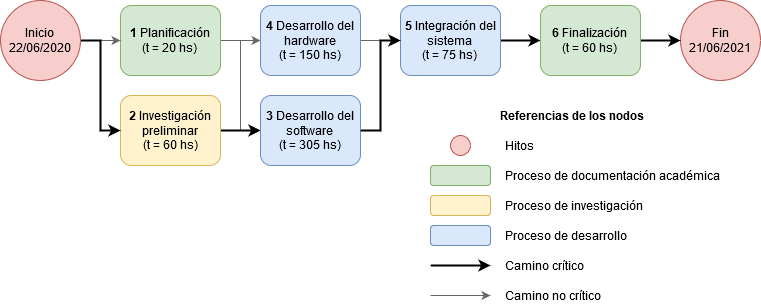
\includegraphics[width=1\textwidth]{./Figuras/activity_on_node.png}
\caption{Diagrama de \textit{Activity on Node}}
\label{fig:AoN}
\end{figure}

\newpage

\section{8. Diagrama de Gantt}
\label{sec:gantt}

Se elaboró el diagrama considerando que se trabajará entre 10 y 20 horas por semana, ajustando el tiempo
donde fuera necesario para cumplir con la fecha de finalización del proyecto. En la tabla siguiente se pueden ver las fechas de
inicio y finalización de cada tarea. En las figuras \ref{fig:gantt1} y \ref{fig:gantt2} se muestra el diagrama de Gantt resultante.

\begin{table}[htpb]
  \centering
  \begin{tabularx}{\linewidth}{@{}|c|X|c|c|@{}}
  \hline
  \rowcolor[HTML]{C0C0C0} 
  WBS  & Nombre de la tarea                                       & Inicio     & Fin        \\ \hline
  1.1  & Elaboración del plan de proyecto                         & 2020-06-22 & 2020-08-09 \\ \hline
  2.1  & Estudio de la documentación original                     & 2020-06-22 & 2020-07-05 \\ \hline
  2.2  & Estudio de la arquitectura y el código fuente original   & 2020-07-06 & 2020-07-19 \\ \hline
  2.3  & Estudio de la normativa                                  & 2020-07-20 & 2020-08-02 \\ \hline
  3.1  & Especificación de requisitos del software                & 2020-08-03 & 2020-08-16 \\ \hline
  3.2  & Especificación de arquitectura del software              & 2020-08-17 & 2020-09-06 \\ \hline
  3.3  & Elaboración del plan de verificación del software        & 2020-09-07 & 2020-09-16 \\ \hline
  3.4  & Elaboración del plan de validación del software          & 2020-09-17 & 2020-09-27 \\ \hline
  3.5  & Selección y configuración del entorno de desarrollo      & 2020-09-28 & 2020-10-01 \\ \hline
  3.6  & Selección de librerías externas                          & 2020-10-02 & 2020-10-08 \\ \hline
  3.7  & Implementación de drivers y primitivas                   & 2020-10-09 & 2020-10-22 \\ \hline
  3.8  & Implementación de módulo de interfaz humano-máquina      & 2020-10-23 & 2020-11-05 \\ \hline
  3.9  & Implementación de módulo de medición de velocidad        & 2020-11-06 & 2020-11-19 \\ \hline
  3.10 & Implementación de módulo de comunicación y localización  & 2020-11-20 & 2020-12-10 \\ \hline
  3.11 & Implementación de módulo de lógica principal             & 2020-12-11 & 2020-12-24 \\ \hline
  3.12 & Pruebas y verificación del software                      & 2020-12-25 & 2020-12-31 \\ \hline
  3.13 & Elaboración de informe de verificación                   & 2021-01-01 & 2021-01-10 \\ \hline
  4.1  & Revisión y actualización de la arquitectura del hardware & 2021-01-11 & 2021-01-17 \\ \hline
  4.2  & Selección de módulos y componentes                       & 2021-01-18 & 2021-01-24 \\ \hline
  4.3  & Actualización de los diagramas esquemáticos              & 2021-01-25 & 2021-01-31 \\ \hline
  4.4  & Diseño del circuito impreso                              & 2021-02-01 & 2021-02-28 \\ \hline
  4.5  & Fabricación del circuito impreso                         & 2021-03-01 & 2021-03-07 \\ \hline
  4.6  & Pruebas y verificación del hardware                      & 2021-03-08 & 2021-03-21 \\ \hline
  5.1  & Integración de módulos constitutivos                     & 2021-03-22 & 2021-03-28 \\ \hline
  5.2  & Pruebas de integración y verificación del sistema        & 2021-03-29 & 2021-04-11 \\ \hline
  5.3 & Pruebas de campo y validación del sistema                 & 2021-04-12 & 2021-04-25 \\ \hline
  5.4 & Elaboración de informe de validación                      & 2021-04-26 & 2021-05-02 \\ \hline
  6.1 & Elaboración del informe de avance                         & 2021-05-03 & 2021-05-09 \\ \hline
  6.2 & Elaboración de la memoria del proyecto                    & 2021-05-10 & 2021-06-13 \\ \hline
  6.3 & Preparación de la presentación final                      & 2021-06-14 & 2021-06-20 \\ \hline
  \end{tabularx}
  \label{tab:gantt}
\end{table}

\begin{figure}[htbp]
\begin{center}
\begin{ganttchart}[
    % hgrid,
    % vgrid={*{6}{draw=none},dotted},   % Solamente dibujar la grilla por semana
    inline,
    x unit=0.7mm,                     % Tamaño de unidad (días)
    time slot format=isodate,
    link bulge=3,                     % Longitud de la vuelta de las flechas
    milestone right shift=5,          % Ancho de los hitos
    bar label font=\small,            % Tamaño de letra de etiquetas en barras
    bar inline label anchor={east}, bar inline label node/.append style={right=2mm} % Etiquetas a la derecha
  ]{2020-06-22}{2021-01-10}
  \gantttitlecalendar{year, month} \\
  \ganttgroup{Planificación}{2020-06-22}{2020-08-09} \\
    \ganttbar{1.1 Elaboración del plan de proyecto}{2020-06-22}{2020-08-09} \\
  \ganttgroup{Investigación}{2020-06-22}{2020-08-02} \\
    \ganttbar{2.1 Estudio de la documentación original}{2020-06-22}{2020-07-05} \\
    \ganttlinkedbar{2.2 Estudio de la arquitectura y el código fuente original}{2020-07-06}{2020-07-19} \\
    \ganttlinkedbar{2.3 Estudio de la normativa}{2020-07-20}{2020-08-02} \\
  \ganttgroup{Desarrollo del software}{2020-08-03}{2021-01-10} \\
    \ganttbar{3.1 Especificación de requisitos del software}{2020-08-03}{2020-08-16} \\
    \ganttlink{elem5}{elem7}
    \ganttlinkedbar{3.2 Especificación de arquitectura del software}{2020-08-17}{2020-09-06} \\
    \ganttlinkedbar{3.3 Elaboración del plan de verificación del soft...}{2020-09-07}{2020-09-16} \\
    \ganttlinkedbar{3.4 Elaboración del plan de validación del ...}{2020-09-17}{2020-09-27} \\
    \ganttlinkedbar{3.5 Selección y configuración del entorno ...}{2020-09-28}{2020-10-01} \\
    \ganttlinkedbar{3.6 Selección de librerías externas}{2020-10-02}{2020-10-08} \\
    \ganttlinkedbar{3.7 Implementación de drivers ...}{2020-10-09}{2020-10-22} \\
    \ganttlinkedbar{3.8 Implementación de m...}{2020-10-23}{2020-11-05} \\  
    \ganttlinkedbar[
      bar inline label anchor={west}, bar inline label node/.append style={left=2mm}  % Etiqueta a la izquierda
    ]{3.9 Implementación de módulo de medición de velocidad}{2020-11-06}{2020-11-19} \\
    \ganttlinkedbar[
      bar inline label anchor={west}, bar inline label node/.append style={left=2mm}  % Etiqueta a la izquierda
    ]{3.10 Implementación de módulo de comunicación y localización}{2020-11-20}{2020-12-10} \\
    \ganttlinkedbar[
      bar inline label anchor={west}, bar inline label node/.append style={left=2mm}  % Etiqueta a la izquierda
    ]{3.11 Implementación de módulo de lógica principal}{2020-12-11}{2020-12-24} \\
    \ganttlinkedbar[
      bar inline label anchor={west}, bar inline label node/.append style={left=2mm}  % Etiqueta a la izquierda
    ]{3.12 Pruebas y verificación del software}{2020-12-25}{2020-12-31} \\
    \ganttlinkedbar[
      bar inline label anchor={west}, bar inline label node/.append style={left=2mm}  % Etiqueta a la izquierda
    ]{3.13 Elaboración de informe de verificación}{2021-01-01}{2021-01-10}
\end{ganttchart}
\end{center}
\caption{Diagrama de Gantt (Primera parte)}
\label{fig:gantt1}
\end{figure}

\begin{figure}[htbp]
\begin{center}
\begin{ganttchart}[
    % hgrid,
    % vgrid={*{6}{draw=none},dotted},   % Solamente dibujar la grilla por semana
    inline,
    x unit=0.7mm,                     % Tamaño de unidad (días)
    time slot format=isodate,
    link bulge=3,                     % Longitud de la vuelta de las flechas
    milestone right shift=5,          % Ancho de los hitos
    bar label font=\small,            % Tamaño de letra de etiquetas en barras
    bar inline label anchor={east}, bar inline label node/.append style={right=2mm} % Etiquetas a la derecha
  ]{2021-01-11}{2021-08-22}
  \gantttitlecalendar{year, month} \\
  \ganttgroup{Desarrollo del hardware}{2021-01-11}{2021-03-21} \\
    \ganttbar{4.1 Revisión y actualización de la arquitectura del hardware}{2021-01-11}{2021-01-17} \\
    \ganttlinkedbar{4.2 Selección de módulos y componentes}{2021-01-18}{2021-01-24} \\
    \ganttlinkedbar{4.3 Actualización de los diagramas esquemáticos}{2021-01-25 }{2021-01-31} \\
    \ganttlinkedbar{4.4 Diseño del circuito impreso}{2021-02-01}{2021-02-28} \\
    \ganttlinkedbar{4.5 Fabricación del circuito impreso}{2021-03-01}{2021-03-07} \\
    \ganttlinkedbar{4.6 Pruebas y verificación del hardware}{2021-03-08}{2021-03-21} \\
  \ganttgroup{Integración del sistema}{2021-03-22}{2021-05-02} \\
    \ganttbar{5.1 Integración de módulos constitutivos}{2021-03-22}{2021-03-28} \\
    \ganttlink{elem6}{elem8}
    \ganttlinkedbar{5.2 Pruebas de integración y verificación del sistema}{2021-03-29}{2021-04-11} \\
    \ganttlinkedbar{5.3 Pruebas de campo y validación del sistema}{2021-04-12}{2021-04-25} \\
    \ganttlinkedbar{5.4 Elaboración de informe de validación}{2021-04-26}{2021-05-02} \\
  \ganttgroup{Procesos de finalización}{2021-05-03}{2021-06-20} \\
    \ganttbar{6.1 Elaboración del informe de avance}{2021-05-03}{2021-05-09} \\
    \ganttlink{elem11}{elem13}
    \ganttlinkedbar[
      bar inline label anchor={west}, bar inline label node/.append style={left=2mm}  % Etiqueta a la izquierda
    ]{6.2 Elaboración de la memoria del proyecto}{2021-05-10}{2021-06-13} \\
    \ganttlinkedbar[
      bar inline label anchor={west}, bar inline label node/.append style={left=2mm}  % Etiqueta a la izquierda
    ]{6.3 Preparación de la presentación final}{2021-06-14}{2021-06-20} \\
    \ganttlinkedmilestone{Presentación pública}{2021-06-21}
\end{ganttchart}
\end{center}
\caption{Diagrama de Gantt (Segunda parte)}
\label{fig:gantt2}
\end{figure}

\newpage

\section{9. Matriz de uso de recursos de materiales}
\label{sec:recursos}

\begin{table}[!htpb]
\begin{center}
  \begin{tabularx}{\linewidth}{@{}|c|X|m{0.8cm}|m{1.4cm}|m{1.3cm}|m{1.1cm}|@{}}
  \hline
  \cellcolor[HTML]{C0C0C0} & \cellcolor[HTML]{C0C0C0} & \multicolumn{4}{c|}{\cellcolor[HTML]{C0C0C0}Recursos requeridos (horas)} \\ \cline{3-6} 
  \multirow{-2}{*}{\cellcolor[HTML]{C0C0C0}WBS} & \multirow{-2}{*}{\cellcolor[HTML]{C0C0C0}\begin{tabular}[c]{@{}c@{}}Nombre de la tarea\end{tabular}} & PC & Prototipo original del SAL/T & Circuito impreso y componentes & Instru- mental \\ \hline
  1.1 & Elaboración del plan de proyecto & 20 & & & \\ \hline
  2.1 & Estudio de la documentación original & 20 & & & \\ \hline
  2.2 & Estudio de la arquitectura y el código fuente original & 30 & 20 & & 10 \\ \hline
  2.3 & Estudio de la normativa & 10 & & & \\ \hline
  3.1 & Elaboración de la especificación de requisitos & 20 & & & \\ \hline
  3.2 & Elaboración de la especificación de arquitectura & 20 & & & \\ \hline
  3.3 & Elaboración del plan de verificación del software & 10 & & & \\ \hline
  3.4 & Elaboración del plan de validación del software & 10 & & & \\ \hline
  3.5 & Selección y configuración del entorno de desarrollo & 10 & & & \\ \hline
  3.6 & Selección de librerías externas & 10 & & & \\ \hline
  3.7 & Implementación de drivers y primitivas & 20 & 20 & & \\ \hline
  3.8 & Implementación de módulo de interfaz humano-máquina & 20 & 20 & & \\ \hline
  3.9  & Implementación de módulo de medición de velocidad & 30 & 30 & & \\ \hline
  3.10 & Implementación de módulo de comunicación y localización & 30 & 30 & & \\ \hline
  3.11 & Implementación de módulo de lógica principal & 30 & 30 & & \\ \hline
  3.12 & Pruebas y verificación del software & 20 & 20 & & 20 \\ \hline
  3.13 & Elaboración de informe de verificación & 5 & & & \\ \hline
  4.1 & Revisión y actualización de la arquitectura del hardware & 20 & & & \\ \hline
  4.2 & Selección de módulos y componentes & 10 & & & \\ \hline
  4.3 & Actualización de los diagramas esquemáticos & 20 & & & \\  \hline
  4.4 & Diseño del circuito impreso & 60 & & & \\ \hline
  4.5 & Fabricación de circuito impreso & 20 & & 20 & \\  \hline
  4.6 & Pruebas y verificación del hardware & 40 & 40 & 40 & 40 \\ \hline
  5.1 & Integración de módulos constitutivos & 10 & 10 & 10 & \\ \hline
  5.2 & Pruebas de integración y verificación del sistema & 20 & 20 & 20 & 20 \\ \hline
  5.3 & Pruebas de campo y validación del sistema & 10 & 10 & 10 & \\ \hline
  5.4 & Elaboración de informe de validación & 5 & & & \\ \hline
  6.1 & Elaboración del informe de avance & 10 & & & \\ \hline
  6.2 & Elaboración de la memoria del proyecto & 40 & & & \\ \hline
  6.3 & Preparación de la presentación final & 10 & & & \\ \hline
  \end{tabularx}
\end{center}
\label{tab:recursos}
\end{table}

\newpage

\section{10. Presupuesto detallado del proyecto}
\label{sec:presupuesto}

A continuación se presentan los costos directos e indirectos del proyecto.

\begin{table}[htpb]
\centering
\begin{tabularx}{\linewidth}{@{}|X|c|r|r|@{}}
\hline
\rowcolor[HTML]{C0C0C0} 
\multicolumn{4}{|c|}{\cellcolor[HTML]{C0C0C0}COSTOS DIRECTOS} \\ \hline
\rowcolor[HTML]{C0C0C0} 
Descripción &
  \multicolumn{1}{c|}{\cellcolor[HTML]{C0C0C0}Cantidad} &
  \multicolumn{1}{c|}{\cellcolor[HTML]{C0C0C0}Valor unitario} &
  \multicolumn{1}{c|}{\cellcolor[HTML]{C0C0C0}Valor total} \\ \hline
Relay de seguridad              & 10       & \$ 2.500 & \$ 25.000  \\  \hline
Otros componentes electrónicos  & N/A      & N/A      & \$ 20.000  \\ \hline
Fabricación de circuito impreso & N/A      & N/A      & \$ 10.000  \\ \hline
Mano de obra                   & 600 horas & \$ 1.000 & \$ 600.000 \\ \hline
\multicolumn{3}{|c|}{SUBTOTAL} & \multicolumn{1}{c|}{\$ 655.000} \\ \hline
\rowcolor[HTML]{C0C0C0} 
\multicolumn{4}{|c|}{\cellcolor[HTML]{C0C0C0}COSTOS INDIRECTOS} \\ \hline
\rowcolor[HTML]{C0C0C0} 
Descripción &
  \multicolumn{1}{c|}{\cellcolor[HTML]{C0C0C0}Cantidad} &
  \multicolumn{1}{c|}{\cellcolor[HTML]{C0C0C0}Valor unitario} &
  \multicolumn{1}{c|}{\cellcolor[HTML]{C0C0C0}Valor total} \\ \hline
20\% del costo directo & N/A & N/A & \$ 131.000 \\ \hline
\multicolumn{3}{|c|}{SUBTOTAL} & \multicolumn{1}{c|}{\$ 131.000 } \\ \hline
\rowcolor[HTML]{C0C0C0}
\multicolumn{3}{|c|}{TOTAL} & \multicolumn{1}{c|}{\$ 786.000} \\ \hline
\end{tabularx}%
\end{table}

\section{11. Matriz de asignación de responsabilidades}
\label{sec:responsabilidades}

En esta sección se presenta la tabla de asignación de responsabilidades.

Referencias:
\begin{itemize}
	\item P = Responsabilidad Primaria
	\item A = Aprobación
	\item I = Informado
	\item C = Consultado
\end{itemize}

\begin{table}[!htpb]
  \centering
  \resizebox{\textwidth}{!}{%
  \begin{tabular}{|c|m{3.5cm}|m{2cm}|m{2cm}|m{2cm}|m{2cm}|m{2cm}|m{2cm}|}
  \hline
  \rowcolor[HTML]{C0C0C0} 
  \cellcolor[HTML]{C0C0C0} &
    \cellcolor[HTML]{C0C0C0} &
    \multicolumn{6}{c|}{\cellcolor[HTML]{C0C0C0}Nombres y roles del proyecto} \\ \cline{3-8} 
  \rowcolor[HTML]{C0C0C0} 
  \cellcolor[HTML]{C0C0C0} &
    \cellcolor[HTML]{C0C0C0} &
    Responsable &
    Orientador &
    Orientador &
    Colaborador &
    Colaborador &
    Cliente \\ \cline{3-8} 
  \rowcolor[HTML]{C0C0C0} 
  \multirow{-3}{*}{\cellcolor[HTML]{C0C0C0}\begin{tabular}[c]{@{}c@{}}WBS\end{tabular}} &
    \multirow{-3}{*}{\cellcolor[HTML]{C0C0C0}Nombre de la tarea} &
    \authorname & \supname & \cosupname & Dr. Ing. Ariel Lutenberg & Ing. Sergio Dieleke & \clientename \\ \hline
    1.1 & Elaboración del plan de proyecto & P & A & A & A & I & I \\ \hline
    2.1 & Estudio de la documentación original & P & C & & & & \\ \hline
    2.2 & Estudio de la arquitectura y el código fuente original & P & & & & & \\ \hline
    2.3 & Estudio de la normativa & P & & & C & & \\ \hline
    3.1 & Elaboración de la especificación de requisitos del software & P & A & A & I & & A \\ \hline
    3.2 & Elaboración de la especificación de arquitectura del software & P & A & A & I & & I \\ \hline
    3.3 & Elaboración del plan de verificación del software & P & A & A & I & & I \\ \hline
    3.4 & Elaboración del plan de validación del software & P & A & A & I & C & A \\ \hline
    3.5 & Selección y configuración del entorno de desarrollo & P & I & I & & & \\ \hline
    3.6 & Selección de librerías externas & P & C & C & & & \\ \hline
    3.7 & Implementación de drivers y primitivas & P & I & I & & & \\ \hline
    3.8 & Implementación de módulo de interfaz humano-máquina & P & I & I & & & \\ \hline
    3.9 & Implementación de módulo de medición de velocidad & P & I & I & & & \\ \hline
    3.10 & Implementación de módulo de comunicación y localización & P & I & I & & & \\ \hline
    3.11 & Implementación de módulo de lógica principal & P & I & I & & & \\ \hline
    3.12 & Pruebas y verificación del software & P & I & I & & & \\ \hline
    3.13 & Elaboración de informe de verificación & P & A & A & & & I \\ \hline
    4.1 & Revisión y actualización de la arquitectura del hardware & P & A & A & I & C & I \\ \hline
    4.2 & Selección de módulos y componentes & P & C & C & & & \\ \hline
    4.3 & Actualización de los diagramas esquemáticos & P & I & I & & & \\  \hline
  \end{tabular}
  }%
\end{table}

\begin{table}[!htpb]
  \centering
  \resizebox{\textwidth}{!}{%
  \begin{tabular}{|c|m{3.5cm}|m{2cm}|m{2cm}|m{2cm}|m{2cm}|m{2cm}|m{2cm}|}  \hline
  \rowcolor[HTML]{C0C0C0} 
  \cellcolor[HTML]{C0C0C0} &
    \cellcolor[HTML]{C0C0C0} &
    \multicolumn{6}{c|}{\cellcolor[HTML]{C0C0C0}Nombres y roles del proyecto} \\ \cline{3-8} 
  \rowcolor[HTML]{C0C0C0} 
  \cellcolor[HTML]{C0C0C0} &
    \cellcolor[HTML]{C0C0C0} &
    Responsable &
    Orientador &
    Orientador &
    Colaborador &
    Colaborador &
    Cliente \\ \cline{3-8} 
  \rowcolor[HTML]{C0C0C0} 
  \multirow{-3}{*}{\cellcolor[HTML]{C0C0C0}\begin{tabular}[c]{@{}c@{}}WBS\end{tabular}} &
    \multirow{-3}{*}{\cellcolor[HTML]{C0C0C0}Nombre de la tarea} &
    \authorname & \supname & \cosupname & Dr. Ing. Ariel Lutenberg & Ing. Sergio Dieleke & \clientename \\ \hline
    4.4 & Diseño del circuito impreso & P & I & I & & & \\ \hline
    4.5 & Fabricación de circuito impreso & P & I & I & & & \\  \hline
    4.6 & Pruebas y verificación del hardware & P & I & I & & & \\ \hline
    5.1 & Integración de módulos constitutivos & P & I & I & & & \\ \hline
    5.2 & Pruebas de integración y verificación del sistema & P & A & A & I & & I \\ \hline
    5.3 & Pruebas de campo y validación del sistema & P & A & A & I & C & A \\ \hline
    5.4 & Elaboración de informe de validación & P & A & A & I & I & A \\ \hline
    6.1 & Elaboración del informe de avance & P & A & A & I & & I \\ \hline
    6.2 & Elaboración de la memoria del proyecto & P & A & A & A & & \\ \hline
    6.3 & Preparación de la presentación final & P & I & I & A & & \\ \hline
  \end{tabular}
  }%
\end{table}

\newpage

\section{12. Gestión de riesgos}
\label{sec:riesgos}

a) Identificación de los riesgos y estimación de sus consecuencias:

Riesgo 1: Cambios en costos de componentes electrónicos importados o nacionales.
\begin{itemize}
\item Severidad (S): 5 (cinco) \\
Severidad media, tendría un impacto en el costo estimado del proyecto.
\item Probabilidad de ocurrencia (O): 8 (ocho) \\
Ocurrencia alta, debido a la situación actual del país. 
\end{itemize}

Riesgo 2: Pérdida de comunicación con los interesados del proyecto.
\begin{itemize}
\item Severidad (S): 8 (ocho) \\
Severidad alta, la comunicación con los interesados es necesaria para verificar requisitos y validar la funcionalidad del sistema.
\item Probabilidad de ocurrencia (O): 5 (cinco) \\
Ocurrencia media, es posible que los interesados no estén disponibles en los tiempos requeridos para el proyecto.
\end{itemize}

\newpage

Riesgo 3: Falta de tiempo para el desarrollo.
\begin{itemize}
\item Severidad (S): 8 (ocho) \\
Severidad alta, puede provocar que el proyecto no se finalice en el plazo establecido.
\item Probabilidad de ocurrencia (O): 6 (seis) \\
Ocurrencia media, el trabajo se realizará fuera del horario laboral del responsable del proyecto.
\end{itemize} 

Riesgo 4: Extensión del tiempo de cuarentena debido al COVID-19.
\begin{itemize}
\item Severidad (S): 5 (cinco) \\
Severidad media, en la primera etapa del proyecto impide realizar pruebas de campo sobre el prototipo que ya está construído. En la segunda etapa
dificultaría las tareas de validación del sistema.
\item Probabilidad de ocurrencia (O): 5 (cinco) \\
Ocurrencia media, se espera que se desarrolle una vacuna y se regularice la situación a nivel mundial antes de llegar a la etapa de validación del proyecto.
\end{itemize}

Riesgo 5: Rotura de computadora personal.
\begin{itemize}
\item Severidad (S): 8 (ocho) \\
Severidad alta, es una herramienta necesaria en todas las etapas del desarrollo.
\item Probabilidad de ocurrencia (O): 1 (uno) \\
Ocurrencia baja, se trata de una computadora adquirida recientemente en periodo de garantía.
\end{itemize}

Riesgo 6: Falla, rotura o perdida de componentes electrónicos.
\begin{itemize}
\item Severidad (S): 6 (seis) \\
Severidad media, tendría un impacto en el costo estimado del proyecto sumado al tiempo de reposición.
\item Probabilidad de ocurrencia (O): 3 (tres) \\
Ocurrencia baja, en condiciones normales no deberían romperse o perderse componentes.
\end{itemize}

Riesgo 7: Pérdida de archivos de documentación, código fuente o archivos de diseño del proyecto.
\begin{itemize}
\item Severidad (S): 9 (nueve) \\
Severidad alta, se perdería el avance realizado provocando un retraso en la finalización del proyecto.
\item Probabilidad de ocurrencia (O): 5 (cinco) \\
Ocurrencia media, puede ser bastante común dependiendo del medio de almacenamiento utilizado.
\end{itemize}

\newpage

b) Tabla de gestión de riesgos: \hfill (El RPN se calcula como RPN=SxO)

\begin{table}[htpb]
\centering
\begin{tabularx}{\linewidth}{@{}|X|c|c|c|c|c|c|@{}}
\hline
\rowcolor[HTML]{C0C0C0} 
Riesgo & S & O & RPN & S* & O* & RPN* \\ \hline
Cambios en costos de componentes electrónicos importados o nacionales                  & 5 & 8 & 40 &  3 &  8 & 24   \\ \hline
Pérdida de comunicación con los interesados del proyecto                               & 8 & 5 & 32 &  - &  - & -    \\ \hline
Falta de tiempo para el desarrollo                                                     & 8 & 6 & 40 &  8 &  3 & 24   \\ \hline
Extensión del tiempo de cuarentena debido al COVID-19                                  & 5 & 5 & 25 &  - &  - & -    \\ \hline
Rotura de computadora personal                                                         & 8 & 1 &  8 &  - &  - & -    \\ \hline
Falla, rotura o perdida de componentes electrónicos                                    & 6 & 3 & 18 &  - &  - & -    \\ \hline
Pérdida de archivos de documentación, código fuente o archivos de diseño del proyecto  & 9 & 5 & 45 &  9 &  1 & 9    \\ \hline
\end{tabularx}%
\end{table}

Criterio adoptado: 
Se tomarán medidas de mitigación en los riesgos cuyos números de RPN sean mayores a 35.

Nota: los valores marcados con (*) en la tabla corresponden luego de haber aplicado la mitigación.

c) Plan de mitigación de los riesgos que originalmente excedían el RPN máximo establecido:

Riesgo 1: Plan de mitigación \\
Se calcula el presupuesto considerando un posible aumento en el costo de los componentes.
\begin{itemize}
\item Severidad (S): 3 (tres) \\
Severidad baja, debido a que se tiene en cuenta en la gestión de recursos materiales de la planificación.
\item Probabilidad de ocurrencia (O): 8 (ocho) \\
Ocurrencia alta, debido a la situación actual del país. 
\end{itemize}

Riesgo 3: Plan de mitigación \\
La gestión de tiempos se hizo teniendo en cuenta la cantidad de horas disponibles por semana para trabajar en el proyecto.
\begin{itemize}
\item Severidad (S): 8 (ocho) \\
Severidad alta, puede provocar que el proyecto no se finalice en el plazo establecido.
\item Probabilidad de ocurrencia (O): 3 (tres) \\
Ocurrencia baja, debido a que se tiene en cuenta en la gestión de tiempos de la planificación.
\end{itemize} 

Riesgo 7: Plan de mitigación \\
Todo el contenido se almacenará en plataformas online (Google Drive, Dropbox, GitHub).
\begin{itemize}
\item Severidad (S): 9 (nueve) \\
Severidad alta, se perdería el avance realizado provocando un retraso en la finalización del proyecto.
\item Probabilidad de ocurrencia (O): 1 (uno) \\
Ocurrencia baja, es muy poco probable que los archivos se pierdan o sean irrecuperables.
\end{itemize}

\section{13. Gestión de la calidad}
\label{sec:calidad}

\begin{consigna}{red}
Tener en cuenta que en este contexto se pueden mencionar simulaciones, cálculos, revisión de hojas de datos, consulta con expertos, etc.
\end{consigna}

\begin{itemize}
\item Req \#1: La interfaz debe contar con una llave rotativa precintable para activar el modo aislado limitado.
\begin{itemize}
  \item Verificación:\\
  Se verificará la hoja de datos de la llave rotativa y se comprobará que cumple con niveles de seguridad adecuados para la aplicación.
  \item Validación:\\
  Se comprobará que con la llave precintada no hay forma de activar el modo aislado, se colocará la llave en la posición AL y se verificará que se enciendan los leds indicadores correspondientes.
\end{itemize}

\item Req \#2: La interfaz debe indicar el estado actual del sistema.
\begin{itemize}
  \item Verificación:\\
  Se hará una prueba que encienda los leds de la interfaz humano-máquina de forma secuencial.
  \item Validación:\\
  Se activará el modo aislado limitado y se verificará que enciendan los leds indicadores correspondientes.
\end{itemize}

\item Req \#3: La interfaz debe mostrar la velocidad media del equipo en km/h con 4 dígitos.
\begin{itemize}
  \item Verificación:\\
  Se hará una prueba que encienda el display de la interfaz humano-máquina y haga un barrido de valores desde cero al límite máximo de velocidad.
  \item Validación:\\
  Se activará el modo aislado limitado y se verificará que se muestre el valor correcto en el display.
\end{itemize}

\item Req \#4: La interfaz debe indicar el estado de la señal de corte de tracción.
\begin{itemize}
  \item Verificación:\\
  Se hará una prueba que encienda los leds de la interfaz humano-máquina de forma secuencial.
  \item Validación:\\
  Se activará el modo aislado limitado y se verificará que enciendan los leds indicadores correspondientes.
\end{itemize}

\item Req \#5: La interfaz debe indicar el estado de la señal de freno de emergencia.
\begin{itemize}
  \item Verificación:\\
  Se hará una prueba que encienda los leds de la interfaz humano-máquina de forma secuencial.
  \item Validación:\\
  Se activará el modo aislado limitado y se verificará que enciendan los leds indicadores correspondientes.
\end{itemize}

\item Req \#6: La interfaz debe indicar la presencia de un comando remoto de la central operativa.
\begin{itemize}
  \item Verificación:\\
  Se hará una prueba que encienda los leds de la interfaz humano-máquina de forma secuencial.
  \item Validación:\\
  Se activará el modo aislado limitado y se verificará que enciendan los leds indicadores correspondientes.
\end{itemize}

\item Req \#7: La interfaz debe indicar el estado de los módulos GPS.
\begin{itemize}
  \item Verificación:\\
  Se hará una prueba que encienda los leds de la interfaz humano-máquina de forma secuencial.
  \item Validación:\\
  Se activará el modo aislado limitado y se verificará que enciendan los leds indicadores correspondientes.
\end{itemize}

\item Req \#8: La interfaz debe indicar el estado de la alimentación.
\begin{itemize}
  \item Verificación:\\
  Se hará una prueba que encienda los leds de la interfaz humano-máquina de forma secuencial.
  \item Validación:\\
  Se activará el modo aislado limitado y se verificará que enciendan los leds indicadores correspondientes.
\end{itemize}

\item Req \#9: El sistema debe informar al registrador de eventos la activación del modo aislado limitado.
\begin{itemize}
  \item Verificación:\\
  Se medirán los contactos de la salida correspondiente y se verificará el cambio de estado cuando se activa el modo aislado limitado.
  \item Validación:\\
  Se conectará el equipo al registrador de eventos Hasler y se comprobará que registra correctamente la activación del modo aislado limitado.
\end{itemize}

\item Req \#10: El sistema debe informar al registrador de eventos si la alimentación es correcta.
\begin{itemize}
  \item Verificación:\\
  Se relizará un ensayo con una fuente de alimentación de laboratorio.
  Se medirán los contactos de la salida correspondiente y se verificará el cambio de estado cuando disminuye la tensión de alimentación fuera del rango aceptable.
  \item Validación:\\
  Se conectará el equipo a una fuente de alimentación de una formación y al registrador de eventos Hasler.
  Se comprobará que registra correctamente que la alimentación está dentro del rango adecuado.
\end{itemize}

\item Req \#11: El sistema debe informar al registrador de eventos la activación del freno de emergencia.
\begin{consigna}{red}
\begin{itemize}
  \item Verificación:\\
  \item Validación:\\
\end{itemize}
\end{consigna}

\item Req \#12: El sistema debe informar al registrador de eventos la activación del corte de tracción.
\begin{consigna}{red}
\begin{itemize}
  \item Verificación:\\
  \item Validación:\\
\end{itemize}
\end{consigna}

\item Req \#13: El sistema debe informar periódicamente (con un tiempo configurable) su estado a la central operativa a través de la red de datos GPRS, 3G ó 4G.
\begin{consigna}{red}
\begin{itemize}
  \item Verificación:\\
  \item Validación:\\
\end{itemize}
\end{consigna}

\item Req \#14: El sistema debe utilizar la antena GPRS/GPS ya disponible en la formación.
\begin{consigna}{red}
\begin{itemize}
  \item Verificación:\\
  \item Validación:\\
\end{itemize}
\end{consigna}

\item Req \#15: Debe existir la posibilidad de usar 2 proveedores distintos de datos de manera simultánea.
\begin{consigna}{red}
\begin{itemize}
  \item Verificación:\\
  \item Validación:\\
\end{itemize}
\end{consigna}

\item Req \#16: El protocolo de comunicación con la central operativa debe ser MQTT.
\begin{consigna}{red}
\begin{itemize}
  \item Verificación:\\
  \item Validación:\\
\end{itemize}
\end{consigna}

\item Req \#17: El sistema debe ser capaz de recibir un comando remoto que anule el corte de tracción y el freno de emergencia bajo cualquier condición (modo aislado total).
\begin{consigna}{red}
\begin{itemize}
  \item Verificación:\\
  \item Validación:\\
\end{itemize}
\end{consigna}

\item Req \#18:  El sistema debe ser capaz de recibir un comando remoto que active el corte de tracción y el freno de emergencia bajo cualquier condición (modo parada total).
\begin{consigna}{red}
\begin{itemize}
  \item Verificación:\\
  \item Validación:\\
\end{itemize}
\end{consigna}

\item Req \#19: El sistema debe ser capaz de recibir un comando remoto que active el corte de tracción y anule el freno de emergencia bajo cualquier condición (modo coche en deriva).
\begin{consigna}{red}
\begin{itemize}
  \item Verificación:\\
  \item Validación:\\
\end{itemize}
\end{consigna}

\item Req \#20: El sistema debe ser capaz de recibir un comando remoto que active el corte de tracción y el freno de emergencia de forma intermitente en ciclos de tiempo configurables (modo intermitente).
\begin{consigna}{red}
\begin{itemize}
  \item Verificación:\\
  \item Validación:\\
\end{itemize}
\end{consigna}

\item Req \#21: El sistema debe ser capaz de recibir un comando remoto que cancele cualquier comando remoto vigente.
\begin{consigna}{red}
\begin{itemize}
  \item Verificación:\\
  \item Validación:\\
\end{itemize}
\end{consigna}

\item Req \#22: El sistema debe ser capaz de recibir comandos remotos que modifiquen sus parámetros internos configurables.
\begin{consigna}{red}
\begin{itemize}
  \item Verificación:\\
  \item Validación:\\
\end{itemize}
\end{consigna}

\item Req \#23: Si no se recibe un nuevo comando remoto luego de un tiempo configurable (por defecto 10 segundos, máximo 1 minuto), debe volver al algoritmo de activación de corte de tracción y freno de emergencia por defecto.
\begin{consigna}{red}
\begin{itemize}
  \item Verificación:\\
  \item Validación:\\
\end{itemize}
\end{consigna}

\item Req \#24: Ante un comando remoto recibido, debe enviar una confirmación de recepción que permita a la central operativa decidir si es necesaria o no una retransmisión.
\begin{consigna}{red}
\begin{itemize}
  \item Verificación:\\
  \item Validación:\\
\end{itemize}
\end{consigna}

\item Req \#25: Debe utilizar algún mecanismo de encriptación para el enlace con la central operativa.
\begin{consigna}{red}
\begin{itemize}
  \item Verificación:\\
  \item Validación:\\
\end{itemize}
\end{consigna}

\item Req \#26: El modo normal el sistema no debe intervenir en el funcionamiento del material rodante (prioridad alta).
\begin{consigna}{red}
\begin{itemize}
  \item Verificación:\\
  \item Validación:\\
\end{itemize}
\end{consigna}

\item Req \#27: El sistema debe ser capaz de recibir la velocidad a partir de una señal digital provista por el registrador de eventos Hasler Teloc 1500. 
\begin{itemize}
  \item Verificación:\\
  Se harán pruebas con un controlador externo que simule las distintas fuentes de velocidad y se verificará el valor mostrado en el display.
  \item Validación:\\
  Se conectará el equipo al registrador de eventos con un generador de impulsos y se verificará el valor mostrado en el display.
\end{itemize}

\item Req \#28: El sistema debe ser capaz de calcular la velocidad a partir de un generador de impulsos ópticos instalado en una o varias ruedas de la formación.
\begin{consigna}{red}
\begin{itemize}
  \item Verificación:\\
  \item Validación:\\
\end{itemize}
\end{consigna}

\item Req \#29: El sistema debe ser capaz de calcular la velocidad a partir de un sistema GPS integrado.
\begin{consigna}{red}
\begin{itemize}
  \item Verificación:\\
  \item Validación:\\
\end{itemize}
\end{consigna}

\item Req \#30: El rango de velocidad soportado por el sistema tiene que estar entre 0 y 120 km/h.
\begin{consigna}{red}
\begin{itemize}
  \item Verificación:\\
  \item Validación:\\
\end{itemize}
\end{consigna}

\item Req \#31: La estimación de velocidad debe tener una precisión del 2\% de fondo de escala. 
\begin{consigna}{red}
\begin{itemize}
  \item Verificación:\\
  \item Validación:\\
\end{itemize}
\end{consigna}

\item Req \#32: En modo aislado limitado el sistema debe evitar la aplicación del corte de tracción.
\begin{consigna}{red}
\begin{itemize}
  \item Verificación:\\
  \item Validación:\\
\end{itemize}
\end{consigna}

\item Req \#33: En modo aislado limitado el sistema debe evitar la aplicación del freno de emergencia.
\begin{consigna}{red}
\begin{itemize}
  \item Verificación:\\
  \item Validación:\\
\end{itemize}
\end{consigna}

\item Req \#34: Ante cualquier error interno, el sistema debe dejar de intervenir en la aplicación del corte de tracción.
\begin{consigna}{red}
\begin{itemize}
  \item Verificación:\\
  \item Validación:\\
\end{itemize}
\end{consigna}

\item Req \#35: Ante cualquier error interno, el sistema debe dejar de intervenir en la aplicación del freno de emergencia.
\begin{consigna}{red}
\begin{itemize}
  \item Verificación:\\
  \item Validación:\\
\end{itemize}
\end{consigna}

\item Req \#36: En modo aislado limitado el sistema debe emitir una señal sonora intermitente a través de un buzzer.
\begin{consigna}{red}
\begin{itemize}
  \item Verificación:\\
  \item Validación:\\
\end{itemize}
\end{consigna}

\item Req \#37: Si al pasar de modo normal a modo aislado limitado no se cuenta con una estimación de velocidad, debe activar el corte de tracción y el freno de emergencia por 30 segundos.
\begin{consigna}{red}
\begin{itemize}
  \item Verificación:\\
  \item Validación:\\
\end{itemize}
\end{consigna}

\item Req \#38: Si se supera una velocidad configurable (por defecto 30 km/h), debe activar el corte de tracción y emitir una señal sonora continua a través de un buzzer.
\begin{consigna}{red}
\begin{itemize}
  \item Verificación:\\
  \item Validación:\\
\end{itemize}
\end{consigna}

\item Req \#39: Si se supera una velocidad configurable (por defecto 36 km/h), debe activar el freno de emergencia.
\begin{consigna}{red}
\begin{itemize}
  \item Verificación:\\
  \item Validación:\\
\end{itemize}
\end{consigna}

\item Req \#40: Una vez aplicado, el corte de tracción debe dejar de aplicarse si la velocidad vuelve a ser menor a una velocidad configurable (por defecto 25 km/h).
\begin{consigna}{red}
\begin{itemize}
  \item Verificación:\\
  \item Validación:\\
\end{itemize}
\end{consigna}

\item Req \#41: Una vez aplicado, el freno de emergencia sólo debe dejar de aplicarse luego de un tiempo configurable (por defecto 30 segundos) desde que se superó el límite.
\begin{consigna}{red}
\begin{itemize}
  \item Verificación:\\
  \item Validación:\\
\end{itemize}
\end{consigna}

\item Req \#42: Si la lectura de velocidad es inválida, debe activar y desactivar el corte de tracción y freno de emergencia de manera alternada en ciclos de tiempo configurables.
\begin{consigna}{red}
\begin{itemize}
  \item Verificación:\\
  \item Validación:\\
\end{itemize}
\end{consigna}

\item Req \#43: El sistema debe utilizar la alimentación presente en el material rodante en el rango de 60 V a 110 V de tensión continua.
\begin{consigna}{red}
\begin{itemize}
  \item Verificación:\\
  \item Validación:\\
\end{itemize}
\end{consigna}

\item Req \#44: Los conectores del equipo deben ser unívocos imposibilitando la conexión incorrecta.
\begin{consigna}{red}
\begin{itemize}
  \item Verificación:\\
  \item Validación:\\
\end{itemize}
\end{consigna}

\item Req \#45: El sistema debe poseer una única placa de circuito impreso con el procesador y periféricos necesarios para el procesamiento de las señales del material rodante.
\begin{consigna}{red}
\begin{itemize}
  \item Verificación:\\
  \item Validación:\\
\end{itemize}
\end{consigna}

\end{itemize}

\section{14. Comunicación del proyecto}
\label{sec:comunicaciones}

El plan de comunicación del proyecto es el siguiente:

% Please add the following required packages to your document preamble:
% \usepackage{graphicx}
% \usepackage[table,xcdraw]{xcolor}
% If you use beamer only pass "xcolor=table" option, i.e. \documentclass[xcolor=table]{beamer}
\begin{table}[htpb]
\centering
\resizebox{\textwidth}{!}{%
\begin{tabular}{|m{3cm}|m{2cm}|m{3cm}|c|m{2cm}|m{2cm}|}
\hline
\rowcolor[HTML]{C0C0C0} 
\multicolumn{6}{|c|}{\cellcolor[HTML]{C0C0C0}PLAN DE COMUNICACIÓN DEL PROYECTO}           \\ \hline
\rowcolor[HTML]{C0C0C0} 
¿Qué comunicar?                                                          & Audiencia                  & Propósito                                                                 & Frecuencia & Método de comunicación                   & Responsable           \\ \hline
Plan de proyecto                                                         & Directores Cliente         & Evaluar la definición de objetivos, alcance y gestión de recursos.        & Una vez    & Correo electrónico                       & Ing. Nahuel Espinosa  \\ \hline  
Avances semanales                                                        & Directores                 & Informar el cumplimiento de tareas, resolver dudas, recibir sugerencias.  & Semanal    & Correo electrónico y/o videoconferencia  & Ing. Nahuel Espinosa  \\ \hline
Especificación de requisitos, plan de validación e informe de validación & Cliente                    & Aprobar la definición de requisitos y su validación.                      & Una vez    & Correo electrónico                       & Ing. Nahuel Espinosa  \\ \hline
Informe de avance                                                        & Directores Cliente         & Informar el estado actual del desarrollo del proyecto.                    & Una vez    & Correo electrónico                       & Ing. Nahuel Espinosa  \\ \hline
Presentación del proyecto final                                          & Directores Cliente Jurado  & Exponer el producto final, detallando su diseño y construcción.           & Una vez    & Audiencia pública                        & Ing. Nahuel Espinosa  \\ \hline
\end{tabular}%
}
\end{table}

\section{15. Gestión de compras}
\label{sec:compras}

\begin{consigna}{red}
En caso de tener que comprar elementos o contratar servicios:
a) Explique con qué criterios elegiría a un proveedor.
b) Redacte el Statement of Work correspondiente.
\end{consigna}

\section{16. Seguimiento y control}
\label{sec:seguimiento}

\begin{consigna}{red}
Para cada tarea del proyecto establecer la frecuencia y los indicadores con los se seguirá su avance y quién será el responsable de hacer dicho seguimiento y a quién debe comunicarse la situación (en concordancia con el Plan de Comunicación del proyecto).

El indicador de avance tiene que ser algo medible, mejor incluso si se puede medir en \% de avance. Por ejemplo,se pueden indicar en esta columna cosas como ``cantidad de conexiones ruteadeas'' o ``cantidad de funciones implementadas'', pero no algo genérico y ambiguo como ``\%'', porque el lector no sabe porcentaje de qué cosa.

\end{consigna}

\begin{table}[!htpb]
\centering
\begin{tabularx}{\linewidth}{@{}|X|X|X|X|X|X|@{}}
\hline
\rowcolor[HTML]{C0C0C0} 
\multicolumn{6}{|c|}{\cellcolor[HTML]{C0C0C0}SEGUIMIENTO DE AVANCE}                                                                       \\ \hline
\rowcolor[HTML]{C0C0C0} 
Tarea del WBS & Indicador de avance & Frecuencia de reporte & Resp. de seguimiento & Persona a ser informada & Método de comunic. \\ \hline
 &  &  &  &  &  \\ \hline
 &  &  &  &  &  \\ \hline
 &  &  &  &  &  \\ \hline
 &  &  &  &  &  \\ \hline
 &  &  &  &  &  \\ \hline
\end{tabularx}%
%}
\end{table}

\section{17. Procesos de cierre}    
\label{sec:cierre}

\begin{consigna}{red}
Establecer las pautas de trabajo para realizar una reunión final de evaluación del proyecto, tal que contemple las siguientes actividades:

\begin{itemize}
\item Pautas de trabajo que se seguirán para analizar si se respetó el Plan de Proyecto original:
 - Indicar quién se ocupará de hacer esto y cuál será el procedimiento a aplicar. 
\item Identificación de las técnicas y procedimientos útiles e inútiles que se utilizaron, y los problemas que surgieron y cómo se solucionaron:
 - Indicar quién se ocupará de hacer esto y cuál será el procedimiento para dejar registro.
\item Indicar quién organizará el acto de agradecimiento a todos los interesados, y en especial al equipo de trabajo y colaboradores:
  - Indicar esto y quién financiará los gastos correspondientes.
\end{itemize}

\end{consigna}


\end{document}
